\documentclass[11pt, a4paper]{article}

% Encoding and fonts
\usepackage[utf8]{inputenc}
\usepackage[T1]{fontenc}
\usepackage{times}

% Page layout
\usepackage{geometry}
\geometry{a4paper, margin=0.85in}
\usepackage{setspace}
\setstretch{1.35}

% Mathematics
\usepackage{amsmath, amssymb}

% Graphics and links
\usepackage{graphicx}
\usepackage[hidelinks]{hyperref}

% TikZ for diagrams
\usepackage{tikz}
\usetikzlibrary{shapes.geometric, arrows.meta, positioning, calc, decorations.pathmorphing, backgrounds, fit, shadows.blur}

% Citations
\usepackage[round, authoryear]{natbib}
\bibliographystyle{plainnat}

% Lists and multicolumn
\usepackage{enumitem}
\setlist{nosep, leftmargin=*}
\usepackage{multicol}

% Title formatting
\usepackage{authblk}

\begin{document}

%% ============================================================================
%% PART I: PERSONAL STATEMENT
%% ============================================================================

\begin{center}
{\LARGE \textbf{Personal Statement}}\\[0.3cm]
{\large Soran Ghaderi}\\[0.1cm]
{\normalsize MSc Artificial Intelligence, University of Essex}\\[0.1cm]
{\normalsize December 2025}
\end{center}

\section*{Motivation}

The question that drives my research is when should a generative model learn globally versus search locally at inference time? This question appears simple but conceals fundamental computational challenges. Training learns a transport map from noise to data. Sampling executes that map. But inference-time refinement---SMC resampling, Langevin corrections, planning over generation orderings---blurs this boundary. The more we refine at inference, the more sampling resembles local training.

This realisation emerged through my research trajectory. During my MSc at Essex, I developed Neural Integration of Iterative Reasoning (NIR), a framework for embedding iterative reasoning into LLM hidden states without fine-tuning. The challenge of propagating information through frozen transformer layers taught me how computation flows through neural architectures and when additional inference-time processing provides value. Later, while building TorchEBM, I implemented various MCMC samplers, score-matching objectives, and SDE/ODE integrators. The practical difficulties of training EBMs in high dimensions forced me to confront the deep connection between learning dynamics and sampling dynamics---they are two views of the same underlying question about measure transport.

My current research at UIUC's Blender Lab has sharpened these questions into a concrete research programme. Working on energy-based transformers for image generation, I am investigating mode collapse in high-dimensional multi-modal spaces. I have developed experimental infrastructure for class-conditional generation, implemented latent caching for rapid iteration, and evaluated architectural variants against diffusion transformer baselines. Simultaneously, I am developing mathematical frameworks for training EBMs with long sampling trajectories while avoiding backpropagation through time, leveraging equilibrium states. This work has convinced me that progress requires theoretical clarity about the learning-sampling-search tradeoff together with practical tools for geometry-aware adaptive transport.

\section*{Research Trajectory and Skills}

My path to this research agenda has been unconventional but coherent. I built substantial engineering infrastructure before focusing on theory, giving me a distinctive perspective on computational constraints that shape algorithmic choices.

\textbf{TorchEBM} (8,000+ downloads) implements energy-based models, diffusion processes, and flow matching in PyTorch. I designed the library around efficient SDE/ODE integration, mixed-precision training, and modular samplers. The next release will include equilibrium matching and new transport schemes motivated by my current theoretical work on avoiding BPTT through implicit differentiation at equilibrium.

\textbf{cuRBLAS} addresses a specific computational bottleneck I encountered. Probabilistic linear algebra operations---trace estimation via Hutchinson's estimator, randomised SVD---arise frequently in sliced score matching but lack optimised GPU implementations. Building CUDA kernels, designing Python bindings, and profiling memory bandwidth taught me how algorithmic choices interact with hardware constraints.

These projects emerged organically from research needs. While studying sliced score matching, I needed efficient Hutchinson trace estimators. While scaling energy-based transformers, I needed custom kernels for EBM-specific attention patterns. This feedback loop between theory and implementation is essential for computationally challenging problems where hardware constraints shape what is tractable.

My mathematical preparation includes optimisation theory, probability, numerical methods, and differential equations. I am comfortable deriving bounds, proving convergence results, and translating theoretical insights into algorithms. My ongoing collaborations with researchers at UIUC, Harvard, and Oxford on implicit gradients for EBMs have strengthened my ability to develop mathematical frameworks from first principles.

\section*{Why Imperial and This Research Direction}

Imperial's strength in combining theoretical depth in generative modelling with serious engagement in scientific applications aligns well with my research direction. The research agenda I propose---developing a unified theory of learning, sampling, and search through information geometry and optimal transport---requires exactly this combination.

Recent advances in the field demonstrate convergence toward this unified view. Sequential Boltzmann Generators combine learned flows with inference-time Langevin dynamics and SMC. Feynman-Kac correctors enable principled composition and guidance through weighted search over diffusion paths. Metric flow matching and Fisher flow matching extend transport to Riemannian manifolds and categorical data. Progressive Inference-Time Annealing enables equilibrium sampling of previously intractable molecular systems. These methods treat learning and sampling as related transport operations, but the field lacks theory explaining when inference-time search becomes necessary and how computation should be allocated.

The problems I want to solve---deriving information-geometric criteria for when search provides value over direct sampling, developing geometry-aware adaptive algorithms, enabling generalisation across target distributions through inference-time search---require collaboration across optimisation, differential geometry, sampling theory, and scientific computing. Imperial's interdisciplinary research environment and computational infrastructure enable the large-scale experiments necessary to validate theoretical predictions.

\section*{Career Aspirations}

My goal is a research career at the frontier of generative modelling, developing both theoretical foundations and practical algorithms. The specific problems I want to work on---adaptive transport, geometry-aware generation, and the learning-sampling-search tradeoff---have applications in molecular design, materials science, and other scientific domains where we can specify energy functions but cannot sample efficiently.

The PhD research I propose would establish theoretical criteria distinguishing when direct sampling suffices from when active search is required, develop geometry-respecting algorithms for adaptive transport, and demonstrate generalisation to new targets through inference-time search without retraining. This combination of theoretical rigour and algorithmic applicability is what I find most compelling about modern machine learning research.

A PhD at Imperial would provide the theoretical depth, collaborative environment, and computational resources necessary to make progress on these challenging problems. I have the preparation in mathematics, systems engineering, and generative modelling to contribute meaningfully from day one.

\newpage

%% ============================================================================
%% PART II: RESEARCH PROPOSAL
%% ============================================================================

\setcounter{section}{0}

\begin{center}
{\LARGE \textbf{Transport as Computation: A Unified Theory of}}\\[0.15cm]
{\LARGE \textbf{Learning, Sampling, and Search in Generative Models}}\\[0.3cm]
{\large Soran Ghaderi}\\[0.1cm]
{\normalsize MSc Artificial Intelligence, University of Essex}\\[0.1cm]
{\normalsize December 2025}
\end{center}

\begin{abstract}
The distinction between learning and sampling in generative models is artificial. Training learns a transport map, sampling executes it, and inference-time refinement learns locally while sampling. When should a generative model search at inference versus directly sample? This proposal develops a unified framework treating learning, sampling, and search as points on a continuous spectrum of measure transport operations, with information geometry determining when search becomes necessary. The central thesis is that optimal generative computation should allocate resources dynamically among global model updates, direct sampling, and inference-time search based on the geometry of the target measure and the complexity of the generation task. Building on advances in flow matching, Schrödinger bridges, SMC-guided diffusion, and discrete planning, I aim to establish theoretical foundations and practical algorithms for geometry-aware adaptive transport that generalises across targets without retraining.
\end{abstract}



\section{Introduction}

Consider sampling from a diffusion model. The learned score provides a global transport direction, but each step locally refines the trajectory. SMC resampling or annealed Langevin dynamics inject additional signal at inference time, using target energy to correct global transport. In discrete domains, path planning algorithms~\citep{fredpathPlanningMasked2025} actively search over generation orderings to improve sample quality. The more we refine or search, the more sampling resembles local training, suggesting the boundary between learning and sampling is not fundamental.

I argue that learning, sampling, and search are three manifestations of measure transport distinguished only by scope and computational budget. Training constructs a global transport map, sampling executes transport from prior to target, and inference-time search performs local exploration when the learned map is insufficient. Recent empirical results support this view. Sequential Boltzmann Generators~\citep{charliescalableEquilibriumSampling2025} achieve state-of-the-art molecular sampling by combining learned flows with inference-time Langevin dynamics and SMC. Progressive Inference-Time Annealing~\citep{taraprogressiveInferencetimeAnnealing2025} enables equilibrium sampling of previously intractable systems. Navigation World Models~\citep{amirnavigationWorldModels2025} demonstrate that learned video generation models can plan trajectories by simulating futures and evaluating goal achievement---combining transport (diffusion-based prediction) with search (trajectory ranking and constraint satisfaction) at inference time. In LLM reasoning, self-consistency voting~\citep{paulacertifiedSelfconsistencyStatistical2025} aggregates multiple inference traces, providing statistical certificates through implicit search over the answer distribution.

The missing piece is theory. When does inference-time search help and when is direct sampling sufficient? How should computation be allocated? This proposal develops that theory, grounded in information geometry and optimal transport.

\section{Central Thesis and Research Questions}

\noindent\textbf{Central Thesis.} Learning, sampling, and search in generative models are instances of measure transport, distinguished by scope (global versus local), substrate (model parameters versus sample trajectories), and information source (training data versus target energy). A unified theory should characterise when direct sampling suffices, when inference-time search becomes necessary, and how to transition between these regimes based on the information geometry of the target measure and the complexity of the generation task.

\begin{figure}[ht]
\centering
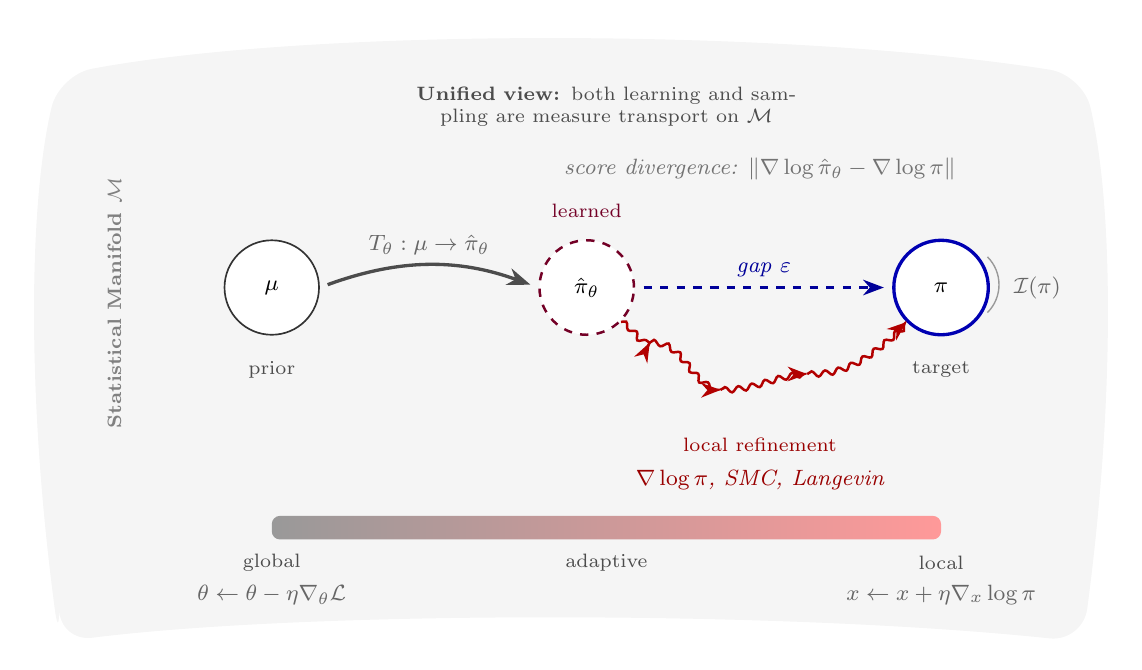
\begin{tikzpicture}[
    >=Stealth,
    % Core styles
    dist/.style={
        circle, draw=black!80, fill=white, line width=0.6pt,
        minimum size=1.2cm, align=center, font=\footnotesize
    },
    manifold/.style={
        draw=none, fill=black!4, rounded corners=12pt
    },
    transport/.style={
        ->, thick, color=#1, line width=1.2pt,
        shorten >=3pt, shorten <=3pt
    },
    localrefine/.style={
        ->, color=#1, line width=0.9pt, 
        decorate, decoration={snake, amplitude=1pt, segment length=5pt}
    },
    annot/.style={font=\scriptsize, text=black!70},
    mathlabel/.style={font=\footnotesize\itshape, text=black!60},
    regionlabel/.style={font=\scriptsize\bfseries, text=black!50}
]

% === BACKGROUND MANIFOLD (Statistical manifold M) ===
\fill[manifold] (-1.2,-4.0) 
    .. controls (2,-3.6) and (8,-3.6) .. (11.8,-4.0)
    .. controls (12.2,-1.0) and (12.2,1.5) .. (11.8,3.2)
    .. controls (8,3.8) and (2,3.8) .. (-1.2,3.2)
    .. controls (-1.6,1.5) and (-1.6,-1.0) .. cycle;

% Manifold label
\node[regionlabel, rotate=90] at (-0.5,0.3) {Statistical Manifold $\mathcal{M}$};

% === DISTRIBUTIONS ===
% Source (prior) - leftmost
\node[dist] (source) at (1.5,0.5) {$\mu$};
\node[annot, below=0.2cm of source] {prior};

% Intermediate (learned approximation) - middle
\node[dist, draw=purple!60!black, dashed, line width=0.9pt] (approx) at (5.5,0.5) {$\hat{\pi}_\theta$};
\node[annot, above=0.15cm of approx, text=purple!60!black] {learned};

% Target - rightmost (with more space)
\node[dist, draw=blue!70!black, line width=1.2pt] (target) at (10,0.5) {$\pi$};
\node[annot, below=0.2cm of target] {target};

% === GLOBAL TRANSPORT (Training: learns T_θ) ===
\draw[transport=black!70] (source.east) 
    to[out=20, in=160] 
    node[above, pos=0.5, mathlabel] {$T_\theta: \mu \to \hat{\pi}_\theta$} 
    (approx.west);

% === TRANSPORT GAP (ε = gap between learned and true) ===
\draw[transport=blue!60!black, dashed, line width=1pt] (approx.east) 
    to[out=0, in=180] 
    node[above, pos=0.5, mathlabel, text=blue!60!black] {gap $\varepsilon$} 
    (target.west);

% === LOCAL REFINEMENT (Inference-time correction) ===
% Clear curved path with Langevin/SMC wiggly arrows below the gap
\coordinate (ref_start) at (6.3,-0.2);
\coordinate (ref_mid1) at (7.2,-0.8);
\coordinate (ref_mid2) at (8.3,-0.6);
\coordinate (ref_end) at (9.3,-0.1);

\draw[localrefine=red!70!black] (approx.south east) to[out=-30, in=180] (ref_start);
\draw[localrefine=red!70!black] (ref_start) to[out=0, in=180] (ref_mid1);
\draw[localrefine=red!70!black] (ref_mid1) to[out=0, in=180] (ref_mid2);
\draw[localrefine=red!70!black] (ref_mid2) to[out=0, in=220] (target.south west);

% Local refinement label - positioned clearly below the path
\node[annot, text=red!60!black, align=center] at (7.7,-1.5) {local refinement};
\node[mathlabel, text=red!60!black] at (7.7,-1.95) {$\nabla \log \pi$, SMC, Langevin};

% === INFORMATION-GEOMETRIC QUANTITIES ===
% Score divergence - positioned above the gap arrow, clearly visible
\node[mathlabel, text=black!55, align=center] at (7.7,2.0) {score divergence: $\|\nabla \log \hat{\pi}_\theta - \nabla \log \pi\|$};

% Fisher information (curvature at target) - positioned to the right of target
\draw[black!40, line width=0.5pt] (target.north east) ++(0.15,-0.05) 
    arc[start angle=45, end angle=-45, radius=0.5cm];
\node[mathlabel, right] at (10.8,0.5) {$\mathcal{I}(\pi)$};

% === SPECTRUM ANNOTATION ===
% Smooth gradient bar with rounded ends (no rectangle overlay)
\shade[left color=black!40, right color=red!40, rounded corners=3pt] 
    (1.5,-2.7) rectangle (10,-2.4);

\node[annot] at (1.5,-3.0) {global};
\node[annot] at (10,-3.0) {local};
\node[annot] at (5.75,-3.0) {adaptive};

% Scope labels - parameter vs sample updates
\node[mathlabel] at (1.5,-3.4) {$\theta \leftarrow \theta - \eta \nabla_\theta \mathcal{L}$};
\node[mathlabel] at (10,-3.4) {$x \leftarrow x + \eta \nabla_x \log \pi$};

% === KEY INSIGHT ANNOTATION ===
\node[annot, text width=6cm, align=center] at (5.75,2.8) {
    \textbf{Unified view:} both learning and sampling are measure transport on $\mathcal{M}$
};

\end{tikzpicture}
\caption{Learning, sampling, and search as measure transport on the statistical manifold $\mathcal{M}$. Training learns a global transport map $T_\theta$ from prior $\mu$ to an approximation $\hat{\pi}_\theta$ of the target $\pi$. The residual gap $\varepsilon$ can be closed through local refinement and search (Langevin dynamics, SMC, planning) using the target score $\nabla \log \pi$. Information-geometric quantities, including score divergence and Fisher information $\mathcal{I}(\pi)$, determine when search provides signal over direct sampling. The spectrum from global parameter updates to local sample trajectory updates represents a continuum of transport operations distinguished by scope and search intensity.}
\label{fig:framework}
\end{figure}

\noindent\textbf{Research Questions.}
\begin{enumerate}
    \item \textbf{When to Search.} What information-geometric quantities (Fisher information, transport cost, score divergence) determine whether direct sampling suffices or inference-time search is required? Can we derive bounds separating regimes where learned transport is accurate from regimes requiring active exploration?
    
    \item \textbf{Geometry-Aware Transport.} How should transport operations respect the intrinsic geometry of the target distribution? Can Riemannian flow matching~\citep{kacpermetricFlowMatching2024, oscargeneralisedFlowMaps2025} be unified with Feynman-Kac correctors~\citep{martafeynmankacCorrectorsDiffusion2025} to yield geometry-preserving adaptive transport?
    
    \item \textbf{Generalisation Across Targets.} Can a transport system trained on one family of targets generalise to new targets using inference-time search alone? What is the role of shared geometric structure in enabling such transfer?
    
    \item \textbf{Search as Computation.} What class of probabilistic computations can be expressed as compositions of learned transport and inference-time search? Does this framework provide a useful abstraction for reasoning, planning, and decision-making in generative models, connecting to multi-step lookahead strategies~\citep{mujineARLBOReinforcementLearning2025, josetransitionConstrainedBayesian2024}?
\end{enumerate}

\noindent\textbf{Aims.}
\begin{enumerate}
    \item Develop a unified theoretical framework connecting training, sampling, and inference-time search through the lens of measure transport and information geometry.
    \item Derive criteria distinguishing when direct sampling is sufficient from when search becomes necessary, based on local target geometry and task complexity.
    \item Design geometry-aware adaptive algorithms that dynamically allocate computation between direct transport and active exploration.
    \item Demonstrate generalisation to new targets through inference-time search, without full retraining.
\end{enumerate}

\section{Literature Review}

\subsection{The Emerging Theory of Transport-Based Generation}

Theory has advanced rapidly. \citet{joeerrorBoundsFlow2024} establish error bounds for flow matching, while \citet{jnearlyDlinearConvergence2024} prove nearly d-linear convergence via stochastic localisation. Score-optimal scheduling~\citep{christopherscoreOptimalDiffusionSchedules2024} derives adaptive discretisation from transport cost. Distributional diffusion~\citep{valentindistributionalDiffusionModels2025} learns posterior distributions for coarse-grained transport. These results characterise training and sampling separately, but do not address when search becomes necessary. My proposal aims to unify all three.

\subsection{Inference-Time Search and SMC}

Recent advances blur the training-sampling boundary through inference-time search. Iterated Denoising Energy Matching~\citep{taraiteratedDenoisingEnergy2024} trains diffusion samplers using only energy evaluations. PITA~\citep{taraprogressiveInferencetimeAnnealing2025} extends this through progressive annealing with Feynman-Kac PDEs. Sequential Boltzmann Generators~\citep{charliescalableEquilibriumSampling2025} combine learned flows with inference-time Langevin dynamics. Feynman-Kac Correctors~\citep{martafeynmankacCorrectorsDiffusion2025} provide principled composition and guidance through weighted search over diffusion paths. Accelerated Parallel Tempering~\citep{leoacceleratedParallelTempering2025} uses neural samplers to reduce overlap requirements while preserving asymptotic guarantees. Particle Denoising Diffusion Sampler~\citep{angusparticleDenoisingDiffusion2024} provides consistent sampling through particle-guided score matching, while Target Score Matching~\citep{valentintargetScoreMatching2024} addresses low-noise score estimation.

\subsection{Geometry-Aware Generative Models}

Standard transport assumes Euclidean geometry, but data lives on lower-dimensional manifolds. Metric Flow Matching~\citep{kacpermetricFlowMatching2024} minimises kinetic energy under data-induced Riemannian metrics. Generalised Flow Maps~\citep{oscargeneralisedFlowMaps2025} extend few-step generation to arbitrary manifolds. Fisher Flow Matching~\citep{oscarfisherFlowMatching2024} enables flow matching for categorical data via Fisher-Rao geometry. Curly Flow Matching~\citep{katarinacurlyFlowMatching2025} handles non-gradient dynamics through Schr\"odinger bridges with drift. Schr\"odinger Bridge Flow~\citep{valentinschrdingerBridgeFlow2024} computes entropy-regularised OT for unpaired translation. Physics-Constrained Fine-Tuning~\citep{janphysicsConstrainedFinetuningFlowmatching2025} incorporates domain structure post-training via PDE residuals. These methods capture geometric structure but do not address when such geometry necessitates search over direct sampling.

\subsection{Discrete Diffusion, Planning, and Search}

Path Planning~\citep{fredpathPlanningMasked2025} decomposes generation into planning and denoising, actively searching over generation orderings. Planner Aware Path Learning~\citep{fredplannerAwarePath2025} derives the Planned ELBO, aligning training with inference-time planning. DDPP~\citep{jarridsteeringMaskedDiscrete2024} steers masked diffusion toward rewards through FK-weighted search. In LLM reasoning, certified self-consistency~\citep{paulacertifiedSelfconsistencyStatistical2025} shows that majority voting over multiple inference traces provides statistical certificates through implicit search over the answer distribution. These methods demonstrate that inference-time search compensates for training-time limitations, but the conditions determining when search is necessary remain unclear.

\subsection{Research Gap}

Existing work treats learning, sampling, and search as separate techniques combined heuristically. The field lacks unified theory explaining when search becomes necessary and predicting its value. Information geometry provides natural tools but has not been systematically applied to this tradeoff. Geometry-aware methods operate in isolation from SMC-based refinement and discrete planning. This proposal bridges these gaps.

\section{Methodology}

\subsection{Phase 1: Information-Geometric Foundations (Year 1)}

Develop theoretical tools characterising the learning-sampling-search tradeoff via three quantities. First, \textbf{score disagreement} measures divergence between learned and target scores, determining when correction or search provides signal. Second, \textbf{local Fisher information} captures target curvature, determining refinement convergence rates and search efficiency. Third, \textbf{transport deficit} quantifies excess cost relative to OT, indicating global error. The central theoretical goal is deriving criteria separating regimes where direct sampling suffices (low disagreement, moderate curvature) from regimes requiring active search (high disagreement, complex geometry). I derive bounds relating these to sample quality, building on~\citet{joeerrorBoundsFlow2024, jnearlyDlinearConvergence2024}, validated on synthetic and molecular systems.

\subsection{Phase 2: Adaptive Transport with Search Allocation (Year 2)}

Current inference-time methods (FKCs, SMC, Langevin) operate in Euclidean space and do not distinguish when search is necessary. This phase develops adaptive algorithms that allocate computation between direct transport and active search based on the criteria from Phase 1. The approach extends FKCs to learned Riemannian manifolds from Metric FM, develops SMC resampling respecting geodesics, and unifies Schrödinger bridges~\citep{valentinschrdingerBridgeFlow2024, katarinacurlyFlowMatching2025} with particle methods~\citep{angusparticleDenoisingDiffusion2024}. Drawing on connections to multi-step lookahead in Bayesian optimization~\citep{mujineARLBOReinforcementLearning2025}, algorithms learn when to commit to direct transport versus when to expand search over alternative trajectories.

\subsection{Phase 3: Generalisation via Inference-Time Search (Year 3)}

Full retraining for each target wastes computation. This phase investigates when inference-time search can substitute for retraining. The approach develops \textbf{meta-transport} maps that generalise across target families (e.g., molecular systems at different temperatures), \textbf{inference-time adaptation} via FKC-style corrections for new targets specified by energy or reward, and \textbf{transfer through shared geometry}. Recent work on visual task vectors~\citep{albertofindingVisualTask2024} and cross-modal task representations~\citep{gracevisionLanguageModelsCreate2025} demonstrates that models can encode task-specific information in compact representations that transfer across modalities and inputs without retraining---providing empirical evidence that inference-time adaptation through learned representations is feasible. The key question is when shared structure enables search-based adaptation versus when retraining is unavoidable. This connects to discrete planning~\citep{fredpathPlanningMasked2025, fredplannerAwarePath2025} and transition-constrained optimization~\citep{josetransitionConstrainedBayesian2024}, where planning at inference time compensates for distributional shift.

\subsection{Phase 4: Compositional Search and Reasoning (Year 4)}

The ultimate test is compositional generation combining transport primitives for unseen targets through structured search. Building on superposition~\citep{martasuperpositionDiffusionModels2024} and product-of-experts via FKCs~\citep{martafeynmankacCorrectorsDiffusion2025}, I investigate when composition yields valid transport, how geometry constrains and enables composition, and whether iterative search constitutes reasoning with predictable convergence. The success of autoregressive visual generation at scale~\citep{yutongsequentialModelingEnables2024} and controllable video prediction conditioned on embodied actions~\citep{amirnavigationWorldModels2025} suggests that compositional transport can extend to high-dimensional visual domains where search over future trajectories enables planning and decision-making. The connection to certified self-consistency~\citep{paulacertifiedSelfconsistencyStatistical2025} suggests that statistical aggregation of search traces can provide formal guarantees on reasoning quality, a direction I will explore for continuous and discrete generation.

\subsection{Evaluation}

\textbf{Theory.} Bounds relating information-geometric quantities to sample quality, following~\citet{jnearlyDlinearConvergence2024}. Convergence in KL/TV decomposed into training error (score approximation) and inference error (discretisation, particles). The goal is identifying regimes where inference-time search provably reduces error beyond additional training, providing a principled answer to when search is necessary.

\textbf{Empirical.} Molecular sampling uses PITA/SBG protocols~\citep{taraprogressiveInferencetimeAnnealing2025, charliescalableEquilibriumSampling2025} on alanine dipeptide and tripeptides. Metrics include energy statistics, ESS per unit time, and MMD against MCMC references. Geometry-aware transport is measured via trajectory length under Riemannian metrics~\citep{kacpermetricFlowMatching2024}. For vision domains, I will evaluate on navigation and trajectory prediction tasks following~\citet{amirnavigationWorldModels2025}, measuring goal achievement under trajectory search versus direct sampling, and quantifying the value of inference-time search in embodied settings. Generalisation experiments test adaptation to held-out temperatures via FKC corrections and, in vision, transfer to novel environments using task-vector-style~\citep{albertofindingVisualTask2024} inference-time steering, quantifying when search enables successful transfer versus when retraining is required.

\section{Risks and Limitations}

\textbf{Geometry estimation cost.} Learning Riemannian metrics~\citep{kacpermetricFlowMatching2024} scales poorly in high dimensions. Mitigation involves focusing on structured domains with moderate intrinsic dimensionality and developing amortised estimation.

\textbf{Bound tightness.} Existing bounds~\citep{joeerrorBoundsFlow2024, jnearlyDlinearConvergence2024} have loose constants. I prioritise testable predictions on tractable benchmarks over asymptotic guarantees.

\textbf{SMC scalability.} Weight degeneracy requires exponential particles in high dimensions. Geometry-aware resampling may help, and I will characterise success regimes and failure modes, particularly when search becomes prohibitively expensive.

\section{Feasibility and Resources}

This proposal builds on open implementations including iDEM, PITA, SBG, Metric/Fisher/Curly FM, and FKCs with established molecular protocols. My TorchEBM library implements EBMs, diffusion, flow matching, and SDE/ODE solvers. The cuRBLAS library provides GPU-accelerated probabilistic linear algebra. Dr.\ Bose's research trajectory from iDEM through PITA to SBG, geometry-aware methods, and discrete planning provides ideal supervision at the intersection of generative modelling, sampling theory, and the emerging theory of inference-time search. Dr.\ Bar's work on navigation world models~\citep{amirnavigationWorldModels2025}, large vision models~\citep{yutongsequentialModelingEnables2024}, and visual task vectors~\citep{albertofindingVisualTask2024} provides complementary expertise in scaling transport-based generation to high-dimensional visual domains and understanding how inference-time search enables planning and generalisation in embodied systems.

\section{Timetable}

\noindent\textbf{Year 1.} Information-geometric foundations and search criteria, months 1--6. Validation on synthetic and molecular benchmarks, months 7--10. First theory paper, months 11--12.

\noindent\textbf{Year 2.} Adaptive transport with search allocation and FKC/SMC integration, months 13--20. Second paper on geometry-respecting inference-time search, months 21--24.

\noindent\textbf{Year 3.} Generalisation across targets via meta-transport and inference-time search, months 25--34. Third paper, months 35--36.

\noindent\textbf{Year 4.} Compositional search experiments, months 37--42. Thesis writing and code release, months 43--48.


{\scriptsize
\setlength{\bibsep}{0pt plus 0.1ex}
\begin{multicols}{2}
\bibliography{imjb-ref,imdocet-ref,imdu-ref,imts-ref,../scholar/imba-ref}
\end{multicols}
}

\end{document}
